\documentclass[11pt]{article}
\usepackage{amssymb}
\usepackage{tipa}
\usepackage{amsmath}
\usepackage[scr]{rsfso}
\usepackage{graphicx}
\usepackage{float}


\newcommand{\then}{\rightarrow} 
\newcommand{\bicond}{\leftrightarrow}
\newcommand{\powerset}[1]{\mathscr{P}(#1)}
\newcommand{\family}[1]{\mathcal{#1}}

\title{\textbf{How to Prove It} \\ {\Large\itshape Daniel J. Velleman} \\ {\Large\itshape Chapter 3.5: Proofs Involving Disjunctions}}

\author{\textbf{Nathaniel Curnick} \\ \textit{Textbook Solutions}}

\date{}

%----------------------------------------------------------------------------------------

\begin{document}

\maketitle

\section*{Exercise 1}

What are the truth sets of the following statements? List a few elements of each 
truth set.

\noindent (a) ``$x$ is a parent of $y$'', where $x$ and $y$ both range of the 
set $P$ of all people 

(Queen Elizabeth, King Charles), (King Charles, Prince William)... 

\noindent (b) ``There is someone who live in $x$ and attends $y$'', where 
$x$ ranges over the set $C$ of all cities and $y$ ranges over the set $U$ of all 
universities.

(Brighton, Sussex), (Oxford, University of Oxford)... 

\section*{Exercise 2}

What are the truth sets of the following statements? List a few elements of each 
truth set.

\noindent (a) ``$x$ lives in $y$'', where $x$ ranges over the set $P$ of all 
people and $y$ ranges over the set $C$ of all cities.

(Prince Chalres, Windsor), (Angelina Jolie, LA)... 

\noindent (b) ``The population of $x$ is $y$'', where $x$ ranges over the set $C$
of all cities and $y$ ranges over $\mathbb{N}$.

(London, 8,000,000), (Paris, 2,000,000)... 

\section*{Exercise 3}

The truth sets of the following statements are subsets of $\mathbb{R}^2$. List a 
few elements of each truth set. Draw a picture showing all the points in the plane 
whose coordinates are in the truth set 

\noindent (a) $y = x^2 - x - 2$

(0,-2), (1,-2), (2,0)... 

\begin{figure}[H]
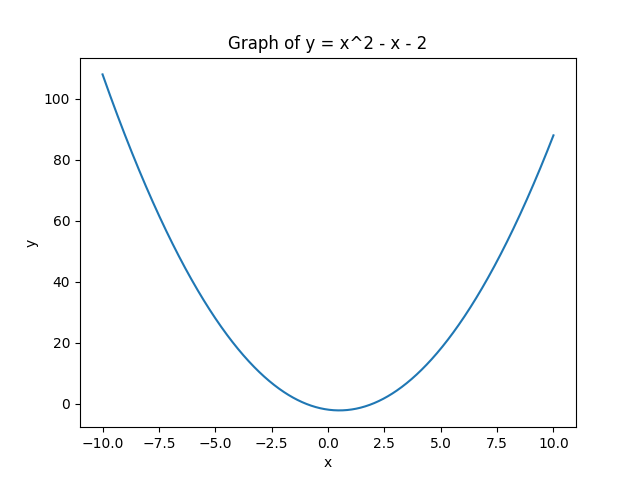
\includegraphics[width=\textwidth]{a.png}
\end{figure}

\noindent (b) $y < x$

(0, -2), (12, 3)... 

\begin{figure}[H]
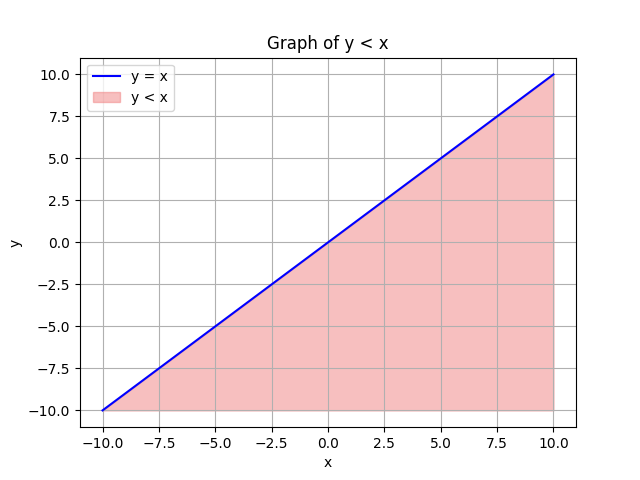
\includegraphics[width=\textwidth]{b.png}
\end{figure}

\noindent (c) Either $y = x^2 - x - 2$ or $y = 3x - 2$

\begin{figure}[H]
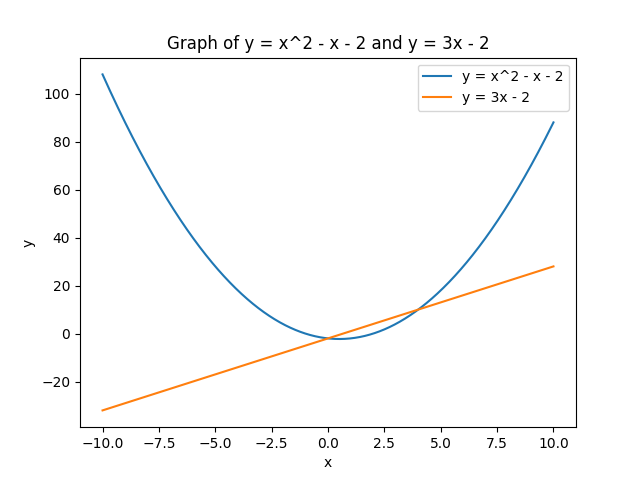
\includegraphics[width=\textwidth]{c.png}
\end{figure}

\noindent (d) $y < x$, and either $y = x^2 - x - 2$ or $y = 3x - 2$

\begin{figure}[H]
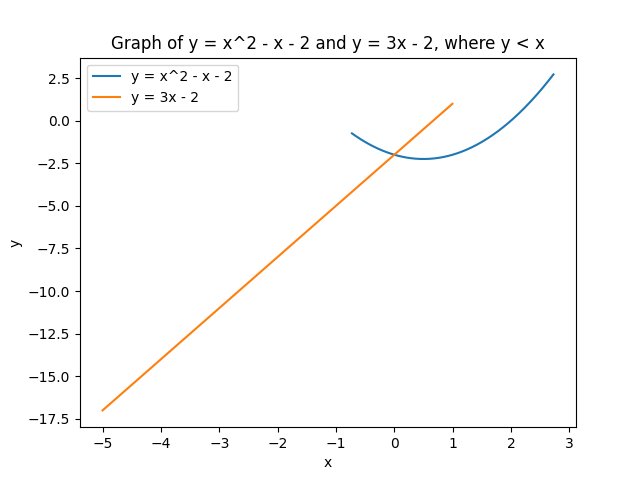
\includegraphics[width=\textwidth]{d.png}
\end{figure}

\section*{Exercise 4}

Let $A = \{ 1,2,3 \}, B = \{ 1, 4 \}, C = \{ 3,4 \}, D = \{ 5 \}$. Compute all 
the sets mentioned in Theorem 4.1.3 and verify that all parts of the theorem 
are true.

We want to demonstrate that $(A \times B) \cap (C \times D) = (A \cap C) \times (B \cap D)$

$$A \times B = \{ (1,1), (1,4), (2,1), (2,4), (3,1), (3,4) \}$$
$$C \times D = \{ (3,5), (4,5) \}$$

So 

$$(A \times B) \cap (C \times D) = \emptyset$$

Now,

$$A \cap C = \{3\}$$
$$B \cap D = \emptyset$$

So, 

$$(A \cap C) \times (B \cap D) = \emptyset$$

So we can see they are verified

\section*{Exercise 5}

Prove parts 2 and 3 of Theorem 4.1.3 

First prove $A \times (B \cup C) = (A \times B) \cup (A \times C)$

Let $p = (x,y)$ be an arbitrary element of $A \times (B \cup C)$. So, $x \in A$ 
and $y \in B \cup C$. Since $y \in B \cup C$ then $y \in B$ or $y \in C$. 
So, $(x,y) \in A \times B$ or $(x,y) \in A \times C$. Thus, 
$(x,y)=(A \times B) \cup (A \times C)$.

Now, let $p$ be an arbitrary element of $(A \times B) \cup (A \times C)$. So, 
$(x, y) \in A \times B$ or $(x, y) \in A \times C$. So, we know that $x \in A$,
the difference is in $y$. $y$ must come from either $B$ or $C$. So, 
$y \in B \cup C$. So, $(x,y) = A \times (B \cup C)$.

Now prove $(A \times B) \cap (C \times D) = (A \cap C) \times (B \cap D)$

Suppose $p = (x,y)$ and $(x,y) \in (A \times B) \cap (C \times D)$. 
So, $(x, y) \in (A \times B)$ and also at the same time $(x,y) \in (C \times D)$.
Thus, $x \in A$ and also $x \in C$. Equally, $y \in B$ and $y \in D$. Thus, 
$(x,y) \in (A \cap C) \times (B \cap D)$.

Suppose now $(x,y) \in (A \cap C) \times (B \cap D)$. So, $x \in A \cap C$ and 
$y \in B \cap D$. Since $x \in A$ and $y \in B$ then $(x,y) \in A \times B$. 
By symmetry, $(x,y) \in C \times D$. So $(x,y) = (A \times B) \cap (C \times D)$.

\section*{Exercise 6}

What's wrong with the following proof that for any sets $A, B, C, D$ that 
$(A \cup C) \times (B \cup D) \subseteq (A \times B) \cup (C \times D)$.

\textit{Proof.} Suppose $(x,y) \in (A \cup C) \times (B \cup D)$. Then 
$x \in A \cup C$ and $y \in B \cup D$, so either $x \in A$ or $x \in C$, and 
either $y \in B$ or $y \in D$. We consider these cases seperately.

Case 1. $x \in A$ and $y \in B$




\end{document}
